\documentclass[15pt,a5paper,reqno]{article}
\usepackage{hyperref}
\usepackage[warn]{mathtext}
\usepackage[utf8]{inputenc}
\usepackage[T2A]{fontenc}
\usepackage[russian]{babel}
\usepackage{amssymb, amsmath, multicol}
\usepackage{graphicx}
\usepackage[shortcuts,cyremdash]{extdash}
\usepackage{wrapfig}
\usepackage{gensymb}
\usepackage{floatflt}
\usepackage{lipsum}
\usepackage{verbatim}
\usepackage{concmath}
\usepackage{euler}
\usepackage{xcolor}
\usepackage{etoolbox}
\usepackage{fancyhdr}
\usepackage{subfiles}
\usepackage{enumitem}
\usepackage{amsthm}
\usepackage{indentfirst}
\usepackage{import}
\usepackage{multirow}
\usepackage{hhline}
\usepackage{calrsfs}

\DeclareMathOperator{\sign}{sign}

\RequirePackage[ left     = 1cm,
                 right    = 1cm,
                 top      = 2.0cm,
                 bottom   = 1.25cm,
                 includefoot,
                 footskip = 1.25cm ]{geometry}
                 
\setlength{\parskip}{ .5em plus .15em minus .08em }
\renewcommand {\baselinestretch}{ 1.07 }

\fancyhf{} % clear existing header/footer entries

\renewcommand{\footrulewidth}{ .0em }
\fancyfoot[C]{\texttt{\textemdash~\thepage~\textemdash}}

\makeatletter
\patchcmd\l@section{%
  \nobreak\hfil\nobreak
}{%
  \nobreak
  \leaders\hbox{%
    $\m@th \mkern \@dotsep mu\hbox{.}\mkern \@dotsep mu$%
  }%
  \hfill
  \nobreak
}{}{\errmessage{\noexpand\l@section could not be patched}}
\makeatother
\parindent = 1cm % отступ при красной строке⏎
\pagestyle{fancy}    
\renewcommand\qedsymbol{$\blacksquare$}

\newcommand{\when}[2]{
  \left. #1 \right|_{#2} \hspace
}
\renewcommand{\kappa}{\varkappa}
\RequirePackage{caption2}
\renewcommand\captionlabeldelim{}
\newcommand*{\hm}[1]{#1\nobreak\discretionary{}

\DeclareSymbolFont{T2Aletters}{T2A}{cmr}{m}{it}
{\hbox{$\mathsurround=0pt #1$}}{}}
% Цвета для гиперссылок
\definecolor{linkcolor}{HTML}{000000} % цвет ссылок
\definecolor{urlcolor}{HTML}{799B03} % цвет гиперссылок
 
\hypersetup{pdfstartview=FitH,  linkcolor=linkcolor,urlcolor=urlcolor, colorlinks=true}


\begin{document}

% НАЧАЛО ТИТУЛЬНОГО ЛИСТА
\begin{center}
  {\small ФЕДЕРАЛЬНОЕ ГОСУДАРСТВЕННОЕ АВТОНОМНОЕ ОБРАЗОВАТЕЛЬНОЕ\\ УЧРЕЖДЕНИЕ ВЫСШЕГО ОБРАЗОВАНИЯ\\ МОСКОВСКИЙ ФИЗИКО-ТЕХНИЧЕСКИЙ ИНСТИТУТ\\ (НАЦИОНАЛЬНЫЙ ИССЛЕДОВАТЕЛЬСКИЙ УНИВЕРСИТЕТ)\\ ФИЗТЕХ-ШКОЛА РАДИОТЕХНИКИ И КОМПЬЮТЕРНЫХ ТЕХНОЛОГИЙ}\\
  \hfill \break
  \hfill \break
  \hfill \break
  \Huge{Работа 3.6.1. \\ Спектральный анализ электрических сигналов}\\
\end{center}

\hfill \break
\hfill \break
\hfill \break
\hfill \break
\hfill \break
\hfill \break
\hfill \break
\hfill \break

\begin{flushright}
  \normalsize{Работу выполнил:}\\
  \normalsize{\textbf{Долгов Александр Алексеевич, группа Б01-106}}\\
\end{flushright}

\begin{center}
  \normalsize{\textbf{Долгопрудный, 2022}}
\end{center}

\thispagestyle{empty} % выключаем отображение номера для этой страницы

% КОНЕЦ ТИТУЛЬНОГО ЛИСТА

\newpage
\thispagestyle{plain}
\tableofcontents
\thispagestyle{plain}
\newpage

\section{Аннотация}

    В данной работе изучается спектральный состав периодических электрических сигналов различной формы: последовательности прямоугольных импульсов, последовательности цугов и амплитудно-модулированных гармонических колебаний. Спектры этих сигналов наблюдались с помощью анализа спектра и сравнивались с рассчитанными теоретически.
	
\section{Теоретические сведения}

    Всякая непрерывная периодическая функция $f(t)$ может быть представлена в виде ряда Фурье:
    \begin{equation*}
        f(t) = \sum\limits_{n = -\infty}^{+\infty} c_n e^{i n \omega_0 t} = \sum\limits_{n = 0}^{+\infty} a_n \cos{(n\omega_0 t + \varphi_n)}
    \end{equation*}
    где $\omega_0 = \frac{2\pi}{T}$, $T$ - период функции $f$. При этом коэффициенты $\{c_n\}$ могу быть найдены по формуле:
    \begin{equation*}
        c_n = \frac{1}{T}\int\limits_{0}^{T} f(t)e^{-i n \omega_0 t} dt
    \end{equation*}
    Также коэффициенты для действительной формы разложения находятся по формулам:
    \begin{equation*}
        a_n = 2|c_n|,\\\ \varphi_n = \arg{c_n}
    \end{equation*}
    
    \begin{wrapfigure}{l}{0.5\textwidth}
        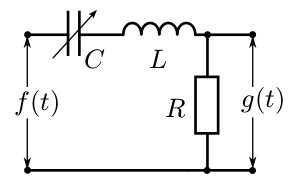
\includegraphics[width=0.5\textwidth]{images/picture_1.png}
        \textbf{Рис. 1. RLC-контур}
    \end{wrapfigure}
    
    \noindentРассмотрим RLC-контур. Для него справедливо второе правило Кирхгофа:
    \begin{equation*}
        L\ddot{q} + R\dot{q} + \frac{q}{C} = e^{i\omega t}
    \end{equation*}
    Входной сигнал - напряжение на резисторе, т.е. $g(t) = R\dot{q}$. Продифференцируем уравнение вынужденных колебаний:
    \begin{equation*}
        L\ddot{I} + R\dot{I} + \frac{I}{C} = i\omega e^{i \omega t}
    \end{equation*}
    \begin{equation*}
        L\frac{\ddot{g}}{R} + \dot{g} + \frac{g}{RC} = i\omega e^{i \omega t}
    \end{equation*}
    \begin{equation*}
        \ddot{g} + \frac{R}{L}\dot{g} + \frac{g}{LC} = i\frac{\omega R}{L} e^{i \omega t}
    \end{equation*}
    Введём обозначения: $\gamma := \frac{R}{2L}$, $\omega_0 := \frac{1}{\sqrt{LC}}$.
    \begin{equation*}
        \ddot{g} + 2\gamma\dot{g} + \omega_0^2 g = i\frac{\omega R}{L} e^{i \omega t}
    \end{equation*}
    Характеристическое уравнение:
    \begin{equation*}
        \lambda^2 + 2\gamma\lambda + \omega_0^2 = 0
    \end{equation*}
    \begin{equation*}
        \lambda = -\gamma \pm \sqrt{\gamma^2 - \omega_0^2}
    \end{equation*}
    Нас интересует лишь случай, когда в контуре возможны колебания, то есть $\gamma < \omega_0$. Таким образом:
    \begin{equation*}
        \lambda = -\gamma \pm i\Omega,\text{ где }\Omega = \sqrt{\omega_0^2 - \gamma^2}
    \end{equation*}
    Тогда общее комплексное решение однородного уравнения имеет вид:
    \begin{equation*}
        g(t) = e^{-\gamma} (A_1 e^{i\Omega t} + A_2 e^{-i\Omega t}),\text{ где }A_1, A_2\in\mathbb{C} 
    \end{equation*}
    Выделим действительные решения:
    \begin{equation*}
        g(t) = e^{-\gamma} (B_1\cos{\Omega t} + B_2 \sin{\Omega t}),\text{ где }B_1, B_2\in\mathbb{R}
    \end{equation*}
    В высокодобротном контуре общее решение однородного уравнения быстро затухнет, и им можно будет пренебречь, говоря, что рассматривается стационарные режим работы контура.
    Частное решение неоднородного уравнения ищем в виде:
    \begin{equation*}
        g(t) = \lambda(\omega)e^{i\omega t}
    \end{equation*}
    \begin{equation*}
        -\omega^2 \lambda + i\cdot 2\gamma\lambda\omega + \omega_0^2\lambda = i\frac{\omega R}{L} e^{i \omega t} \implies \lambda(\omega) = \frac{i\omega R}{L(\omega_0^2 -\omega^2 + i\cdot 2\gamma\omega)}
    \end{equation*}
    \begin{equation*}
        \lambda(\omega) = \frac{\omega R(2\gamma\omega + i(\omega_0^2 -\omega^2))}{L((\omega_0^2 -\omega^2)^2 + 4\gamma^2\omega^2)}
    \end{equation*}
    Окончательно получаем:
    \begin{equation}
        |\lambda(\omega)| = \frac{\omega R}{L}\frac{1}{\sqrt{(\omega_0^2 -\omega^2)^2 + 4\gamma^2\omega^2}}
    \end{equation}
    \begin{equation}
        \varphi(\omega) = \arctg{\frac{2\gamma\omega}{\omega^2 - \omega_0^2}}
    \end{equation}
    Найдём максимум функции $|\lambda (\omega)|$:
    \[\frac{L}{R}\frac{d}{d\omega}(|\lambda (\omega)|) = \frac{(\omega_0^2 -\omega^2)^2 + 4\gamma^2\omega^2 - \omega(-2(\omega_0^2 - \omega^2)\omega + 4\gamma^2\omega)}{((\omega_0^2 -\omega^2)^2 + 4\gamma^2\omega^2)^{3/2}} = \]
    \[= \frac{(\omega_0^2 -\omega^2)^2 + 4\gamma^2\omega^2 + 2(\omega_0^2 - \omega^2)\omega^2 - 4\gamma^2\omega^2}{((\omega_0^2 -\omega^2)^2 + 4\gamma^2\omega^2)^{3/2}} =\]
    \[= \frac{(\omega_0^2 -\omega^2)(\omega_0^2 + \omega^2)}{((\omega_0^2 -\omega^2)^2 + 4\gamma^2\omega^2)^{3/2}} \implies \frac{d}{d\omega}(|\lambda (\omega)|) = 0 \iff \omega = \omega_0\]
    Таким образом, величина $|\lambda(\omega)|$ достигает максимума при $\omega = \omega_0$. Так как $|\lambda(\omega)|$ - коэффициент пропорциональности между входным и выходным сигналами, то делаем вывод, что рассматриваемый колебательный контур усиливает лишь частоты, близкие к резонансной. С точки зрения преобразования гармоник контур является узкополосным фильтром с шириной пропускания порядка
    \begin{equation*}
        \Delta\omega \sim \frac{\omega_0}{Q},\text{ где } Q = \frac{1}{R}\sqrt{\frac{L}{C}} - \text{добротность контура}
    \end{equation*}
    Поскольку амплитуда колебаний в контуре пропорциональна амплитуде гармоники в спектре функции $f(t)$, то, меняя резонансную частоту контура, можно исследовать весь спектр входящего сигнала.

    У описанной выше схемы есть существенный недостаток: при изменении $L$ или $C$ меняется также и добротность, а значит, и ширина полосы пропускания. Кроме того, проще изготовить высокодобротный контур с фиксированными параметрами, нежели с настраиваемой частотой.
    В связи с этим, как правило, для фильтрации сигнала применяется другая схема.

    Отметим также, что для периодических сигналов существует связь между длительностью сигнала ($\Delta t$) и шириной его спектра ($\Delta\nu$):
    \begin{equation}\label{uncertainty}
        \Delta\nu \cdot \Delta t = 1
    \end{equation}
    
\newpage
\section{Экспериментальная установка}

    \hypertarget{pic_2}{\begin{wrapfigure}{l}{0.6\textwidth}
        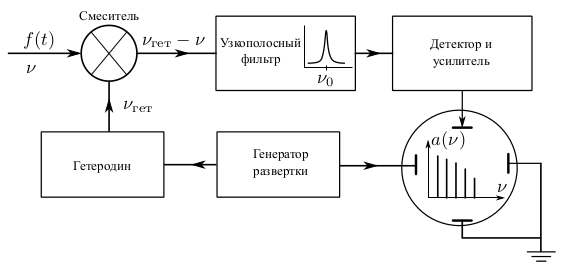
\includegraphics[width=0.6\textwidth]{images/picture_2.png}
        \textbf{Рис. 2. Экспериментальная установка}
    \end{wrapfigure}}
    \noindentСхема экспериментальной установки изображена на Рисунке 2. Исследуемый сигнал $f(t)$ и синусоидальный сигнал от вспомогательного генератора, называемого \textit{гетеродином}, подаются на вход \textit{смесителя} - элемента, преобразующего колебания с частотами $\nu_1$ и $\nu_2$ в колебания на комбинированных частотах: $\nu_1 + \nu_2$ и $\nu_1 - \nu_2$ . Разностный сигнал смесителя поступает на фильтр - высокодобротный колебательный контур, настроенный на некоторую фиксированную резонансную частоту $\nu_0$ . Таким образом, если $f(t)$ содержит гармонику $\nu = \nu_{\text{гет}} - \nu_0$ ($\nu_{\text{гет}}$ - частота гетеродина), она будет усилена, а отклик будет пропорционален её амплитуде. Отметим, что смешение частот исследуемого сигнала и частоты гетеродина лежит в основе большинства современных радиоприёмных устройств — супергетеродинов.

    В спектральном анализаторе частота гетеродина пропорциональна напряжению, подаваемому на развёртку по оси $X$ встроенного в анализатор осциллографа. Выходной сигнал подаётся на канал $Y$ . На экране анализатора возникает, таким образом, график, изображающий зависимость амплитуды гармоник исходного сигнала от частоты, т. е. его спектр (информация о фазах гармоник при этом теряется).
    
\section{Измерения и обработка их результатов}

    Погрешности прямых измерений в данной работе считаются пренебрежимо малыми.

    \subsection{Исследование спектра периодической последовательности прямоугольных импульсов}

        Введём некоторые используемые далее обозначения: $\nu_{\text{повт}}$ - частота повторения импульсов, $T = (\nu_{\text{повт}})^{-1}$; $\tau$ - длительность одного импульса; $\delta\nu$ - расстояние между соседними гармониками (частота первой гармоники); $\Delta\nu$ - ширина спектра (расстояние от главного максимума до первого нуля огибающей).
        \begin{center}
            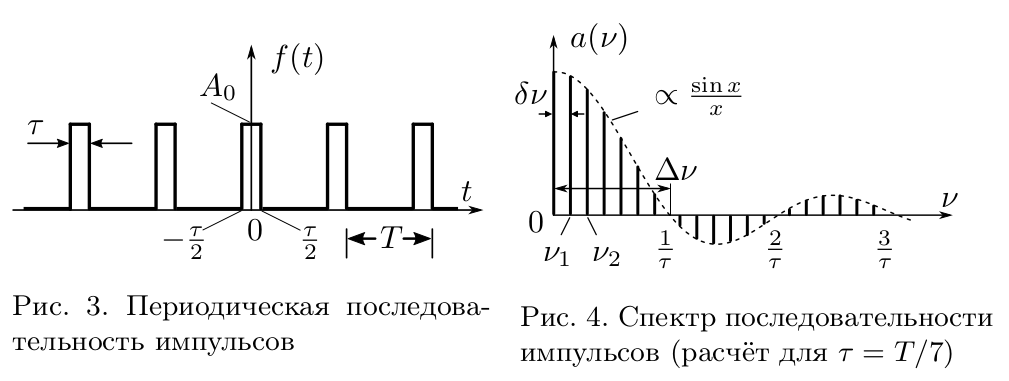
\includegraphics[width = \textwidth]{images/picture_3.png}
        \end{center}

        При изменении параметров сигнала $(\nu_{\text{повт}}, \tau)$ его спектр меняется. В ходе работы было рассмотрено 3 случая: 1) $(\nu_{\text{повт}}, \tau) = (1\text{ кГц}, 100\text{ мкс})$, 2) $(\nu_{\text{повт}}, \tau) = (2\text{ кГц}, 100\text{ мкс})$, 3) $(\nu_{\text{повт}}, \tau) = (1\text{ кГц}, 200\text{ мкс})$. При переходе от параметров 1 к параметрам 2 ширина спектра уменьшается в 2 раза. При переходе от параметров 1 к параметрам 3 расстояние между соседними гармониками $\delta\nu$ увеличивается в 2 раза.

        Далее была измерена зависимость ширины спектра от длительности импульсов при постоянной частоте повторения импульсов $\nu_{\text{повт}}$ = 1 кГц. Результаты представлены в \hyperlink{table_1}{Таблице 1}. По ним также построен \hyperlink{graph_1}{График 1}, позволяющий. Из соотношения неопределённости \eqref{uncertainty} следует, что угловой коэффициент наклона прямой должен быть порядка 1000, что, как видно из графика, выполняется в хорошей точностью.

        Затем были проведены непосредственные измерения спектров при $\tau = 50\text{ мкс}$ и $\tau = 50\text{ мкс}$. Результаты представлены в \hyperlink{table_2}{Таблице 2} ($U_m$ - амплитуда сигнала). По ним построены \hyperlink{graph_2}{График 2} и \hyperlink{graph_3}{График 3}.

    \subsection{Исследование спектра периодической последовательности цугов гармонических колебаний}

        При увеличении длительности импульса $\tau$ вдвое от 100 до 200 мкс ширина спектра уменьшается, а высота увеличивается вдвое. Если же менять несущую частоту $\nu_0$, то вид спектра не меняется, а лишь параллельно переносится вдоль оси абсцисс.

        Далее в работе измерялось расстояние между соседними гармониками при различных частотах повторения цугов. Длительность импульса $\tau$ была установлена в 100 мкс, и измерения проводились для $\nu_{\text{повт}} = 0.5, 1, 2, 4, 5$ кГц. В каждом из измерений оказалось, что $\delta\nu = \nu_{\text{повт}}$. Таким образом, результат соответствует соотношению неопределённости \eqref{uncertainty}.

        Затем были проведены непосредственные измерения спектров при $\tau = 100\text{ мкс}$, $\nu_{\text{повт}}$ = 1 кГц и $\tau = 100\text{ мкс}$, $\nu_{\text{повт}}$ = 2 кГц. Результаты представлены в \hyperlink{table_3}{Таблице 3} ($U_m$ - амплитуда сигнала). По ним построены \hyperlink{graph_4}{График 4} и \hyperlink{graph_5}{График 5}.

    \subsection{Исследование спектра амплитудно-модулированных гармонических сигналов}

        На канал 2 осциллографа подавался синусоидальный сигнал с двойной амплитудой 1 В и частотой $\nu_0$ = 25 кГц (несущая частота). На канал 1 осциллографа подавался синусоидальный сигнал с двойной амплитудой 0.2 В, частотой $\nu_{\text{мод}}$ = 1 кГц (частота модуляции) и смещением на 1 В. В работе измерялись максимальная $A_{max}$ и минимальная $A_{min}$ амплитуды результирующих колебаний, а также амплитуды $A_{\text{осн}}$ и $A_{\text{бок}}$ несущего колебания и боковых гармоник, соответственно. По этим данным находилась глубина модуляции $m = (A_{max} - A_{min})/(A_{max} + A_{min})$ и отношение амплитуд спекьральных составляющих колебаний $k = A_{\text{бок}}/A_{\text{осн}}$. При этих измерениях двойная амплитуда канала 1 изменялась от 0.2 В до 2 В. Результаты измерений представлены в \hyperlink{table_4}{Таблице 4}. Также построен график зависимости $k(m)$ (\hyperlink{graph_6}{График 6}).

        Аппроксимацией точек графика 6 получаем, что $\frac{k}{m} = 0.484 \approx 0.5$, что соответствует теоретическим выводам.
    
\section{Вывод}

    В ходе работы были изучены спектры некоторых периодических сигналов и проверены соотношения, их описывающие, в частности, соотношение неопределённости. Исследованы амплитудно-модулированные сигналы, для которых проверено справедливость теоретического вывода о связи глубины модуляции с отношением амплитуд боковых и несущего колебаний.
    
\newpage
\section{Приложения}

    \subsection{Таблицы}

        \noindent\hypertarget{table_1}{\textbf{Таблица 1. Зависимость ширины спектра от длительности импульса при частоте повторения импульсов 1 кГц.}}
        \begin{center}
            \begin{tabular}{|c|c|c|c|c|c|c|c|c|c|}
                \hline
                $\tau$, мкс      & 40 & 60   & 80   & 100 & 120 & 140 & 160 & 180 & 200 \\ \hline
                $\Delta\nu$, кГц & 25 & 17.5 & 12.5 & 10  & 8   &   7 &   6 & 5.5 & 5   \\ \hline
            \end{tabular}
        \end{center}

        \noindent\hypertarget{table_2}{\textbf{Таблица 2. Спектр сигналов с длительностью одного импульса 50 и 100 мкс}}
        \begin{center}
            \begin{tabular}{|c|c|c|c|c|}
                 \hline
                             & \multicolumn{2}{|c|}{$\tau$ = 50 мкс} & \multicolumn{2}{|c|}{$\tau$ = 100 мкс} \\ \hline\hline
                 № гармоники &      $\nu$, кГц & $U_m$, мВ           &      $\nu$, кГц & $U_m$, мВ            \\ \hline
                        0    &              0  & 148.6               &               0 & 251.4 \\ \hline
                        1    &              1  & 70.15               &               1 & 139.1 \\ \hline
                        2    &              2  & 68.9                &               2 & 129.7 \\ \hline
                        3    &              3  & 67.67               &               3 & 118.4 \\ \hline
                        4    &              4  & 64.19               &               4 & 102.1 \\ \hline
                        5    &              5  & 60.11               &               5 & 83.9 \\ \hline
                        6    &              6  & 56.3                &               6 & 65.71 \\ \hline
                        7    &              7  & 52.8                &               7 & 47.51 \\ \hline
                        8    &              8  & 47.32               &               8 & 29.32 \\ \hline
                        9    &              9  & 42.95               &               9 & 13.64 \\ \hline
                        10   &             10 & 40.32                &              10 & 0 \\ \hline
                        11   &             11 & 37.62                & &\\ \hline
                        12   &             12 & 33.32                & &\\ \hline
                        13   &             13 & 29.38                & &\\ \hline
                        14   &             14 & 25.44                & &\\ \hline
                        15   &             15 & 20.63                & &\\ \hline
                        16   &             16 & 16.03                & &\\ \hline
                        17   &             17 & 11.44                & &\\ \hline
                        18   &             18 & 7.716                & &\\ \hline
                        19   &             19 & 3.777                & &\\ \hline
                        20   &             20 & 0                    & &\\ \hline
            \end{tabular}
        \end{center}

        \noindent\hypertarget{table_3}{\textbf{Таблица 3. Спектр цугов с частотой повторения 1 и 2 кГц}}
        \begin{center}
            \begin{tabular}{|c|c|c|c|c|}
                 \hline
                             & \multicolumn{2}{|c|}{$\nu_{\text{повт}}$ = 50 мкс} & \multicolumn{2}{|c|}{$\nu_{\text{повт}}$ = 100 мкс} \\ \hline\hline
                 № гармоники &      $\nu$, кГц & $U_m$, мВ           &      $\nu$, кГц & $U_m$, мВ            \\ \hline
                      -10    &              20  & 0                  & &\\ \hline
                       -9    &              21  & 7.59               & &\\ \hline
                       -8    &              22  & 15.49              & &\\ \hline
                       -7    &              23  & 24.21              & &\\ \hline
                       -6    &              24  & 31.43              & &\\ \hline
                       -5    &              25  & 41.15              & 20 & 0 \\ \hline
                       -4    &              26  & 45.23              & 22 & 30.48 \\ \hline
                       -3    &              27  & 52.76              & 24 & 63.11 \\ \hline
                       -2    &              28  & 54.01              & 26 & 91.34 \\ \hline
                       -1    &              29  & 59.97              & 28 & 107.6 \\ \hline
                        0    &             30 & 68.75                & 30 & 124.6 \\ \hline    
                        1    &             31 & 58.09                & 32 & 99.49 \\ \hline
                        2    &             32 & 49.93                & 34 & 75.65 \\ \hline
                        3    &             33 & 48.08                & 36 & 48.68 \\ \hline
                        4    &             34 & 38.33                & 38 & 22.33 \\ \hline
                        5    &             35 & 35.82                & 40 & 0 \\ \hline
                        6    &             36 & 24.52                & &\\ \hline
                        7    &             37 & 20.13                & &\\ \hline
                        8    &             38 & 10.72                & &\\ \hline
                        9    &             39 & 5.39                 & &\\ \hline
                       10    &             40 & 0                    & &\\ \hline
            \end{tabular}
        \end{center}

        \noindent\hypertarget{table_4}{\textbf{Таблица 4. Амплитудная модуляция}}
        \begin{center}
            \begin{tabular}{|c|c||c|c|c|c|c|}
                \hline
                $A_1$, В & $A_{max}$, мВ & $A_{min}$, мВ & $A_{\text{осн}}$, мВ & $A_{\text{бок}}$, мВ & m & k\\ \hline\hline
                0.2 & 549.3 & 448.9 & 324   & 14.69 & 0.101 & 0.045 \\ \hline
                0.5 & 619.6 & 373.7 & 324   & 39.16 & 0.248 & 0.121 \\ \hline
                0.8 & 687.3 & 305.9 & 324   & 63    & 0.384 & 0.194 \\ \hline
                1.1 & 762.6 & 230.6 & 324   & 88.09 & 0.536 & 0.272 \\ \hline
                1.4 & 845.4 & 155.3 & 324.6 & 113.2 & 0.690 & 0.349 \\ \hline
                1.7 & 920.7 & 82.57 & 324.6 & 132.3 & 0.835 & 0.408 \\ \hline
                2   & 1008  & 74.69 & 349.2 & 141.4 & 0.862 & 0.405 \\ \hline
            \end{tabular}
        \end{center}

    \newpage
    \subsection{Графики}

        \noindent\hypertarget{graph_1}{\textbf{График 1. Зависимость ширины спектра от длительности импульса при частоте повторения импульсов 1 кГц.}}
        \begin{center}
            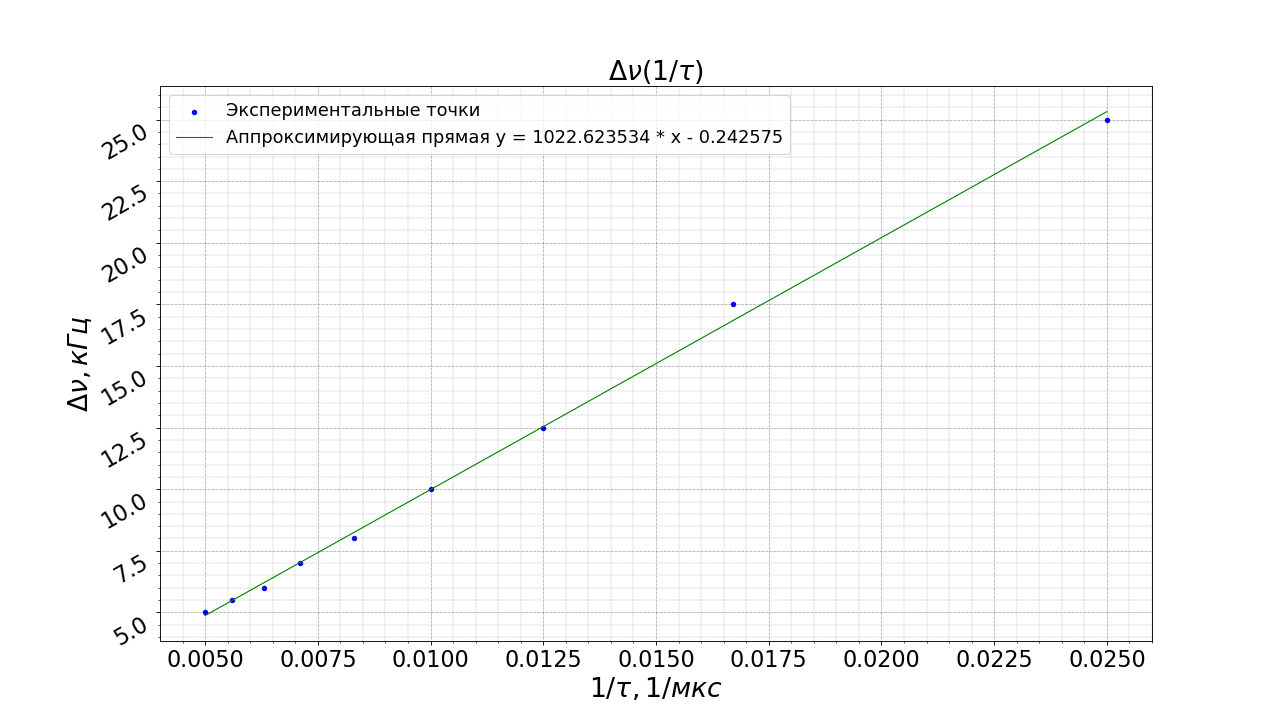
\includegraphics[width = 0.9\textwidth]{images/graph_1.png}
        \end{center}

        \noindent\hypertarget{graph_2}{\textbf{График 2. Спектр прямоугольных сигналов при $\tau$ = 50 мкс}}
        \begin{center}
            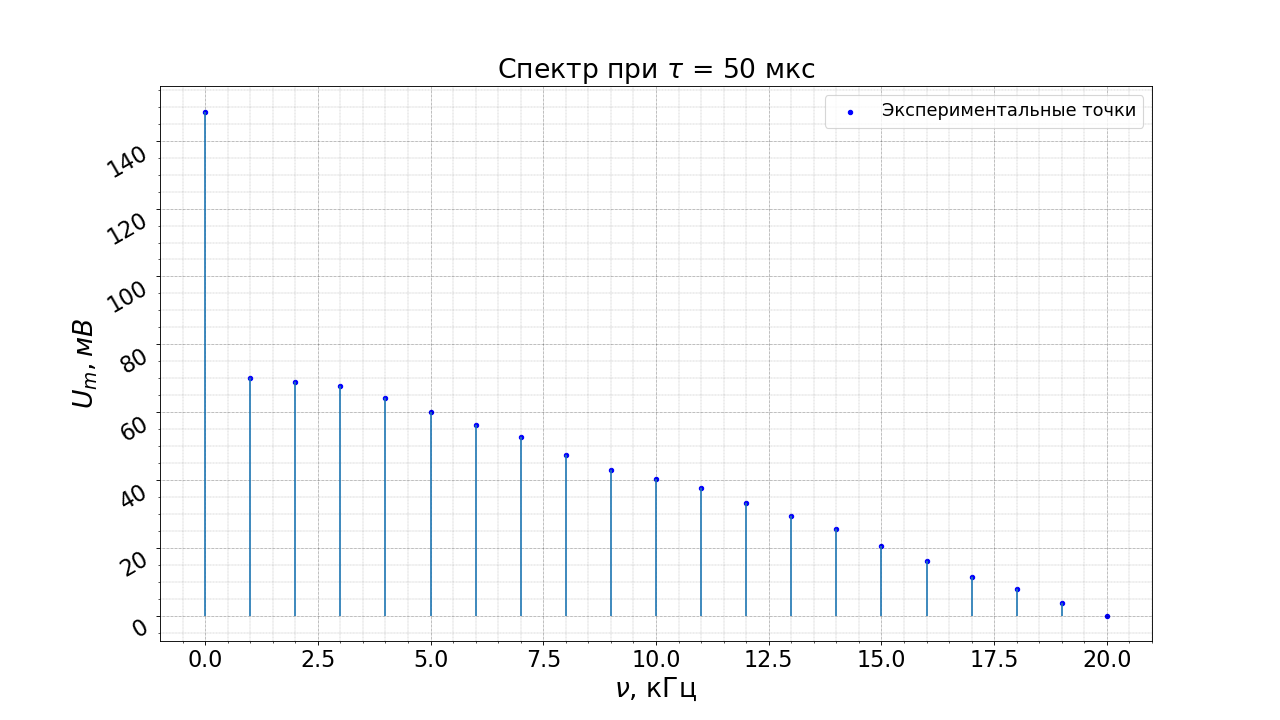
\includegraphics[width = 0.9\textwidth]{images/graph_2.png}
        \end{center}

        \noindent\hypertarget{graph_3}{\textbf{График 3. Спектр прямоугольных сигналов при $\tau$ = 100 мкс}}
        \begin{center}
            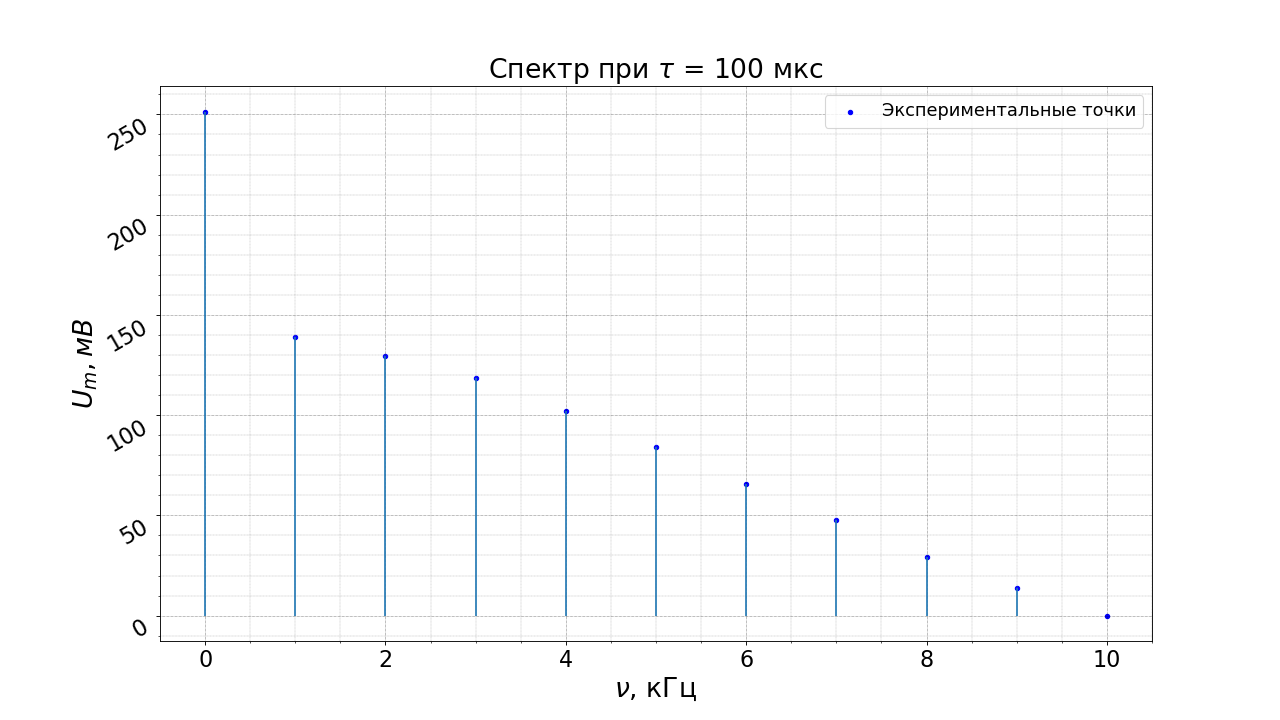
\includegraphics[width = \textwidth]{images/graph_3.png}
        \end{center}

        \noindent\hypertarget{graph_4}{\textbf{График 4. Спектр цугов при $\nu_{\text{повт}}$ = 1 кГц}}
        \begin{center}
            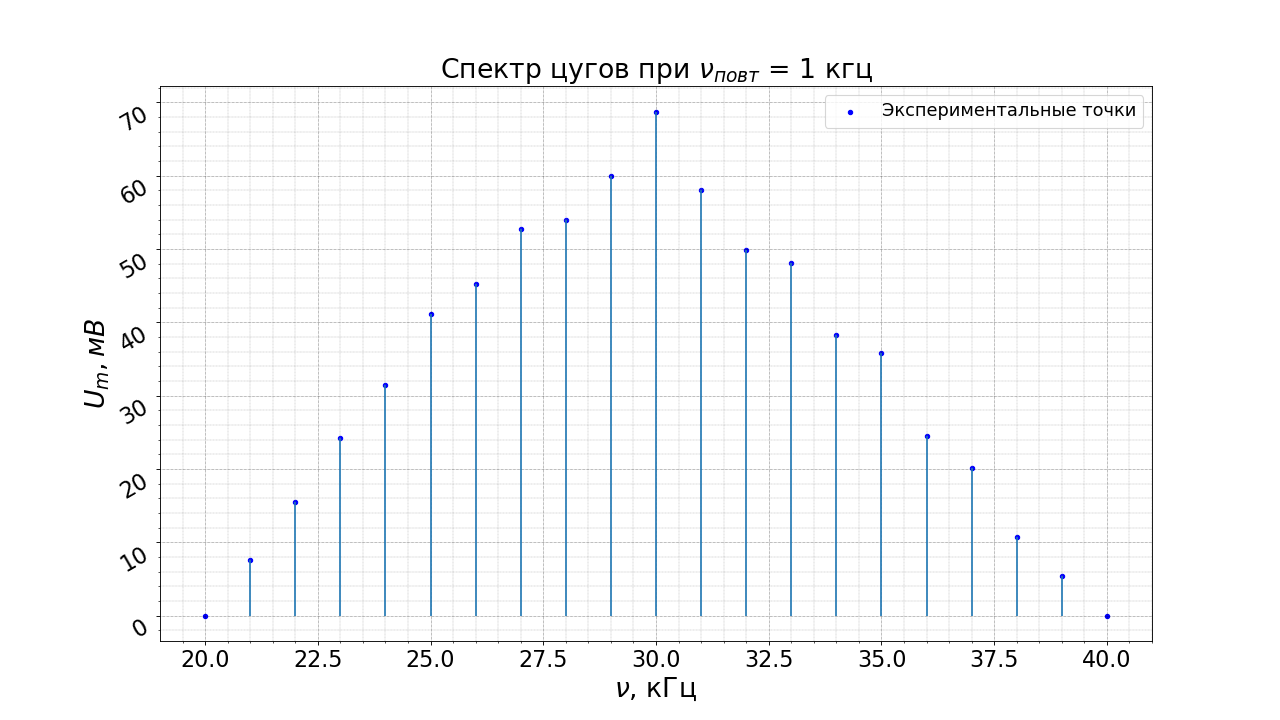
\includegraphics[width = \textwidth]{images/graph_4.png}
        \end{center}

        \noindent\hypertarget{graph_5}{\textbf{График 5. Спектр цугов при $\tau$ = 1 кГц}}
        \begin{center}
            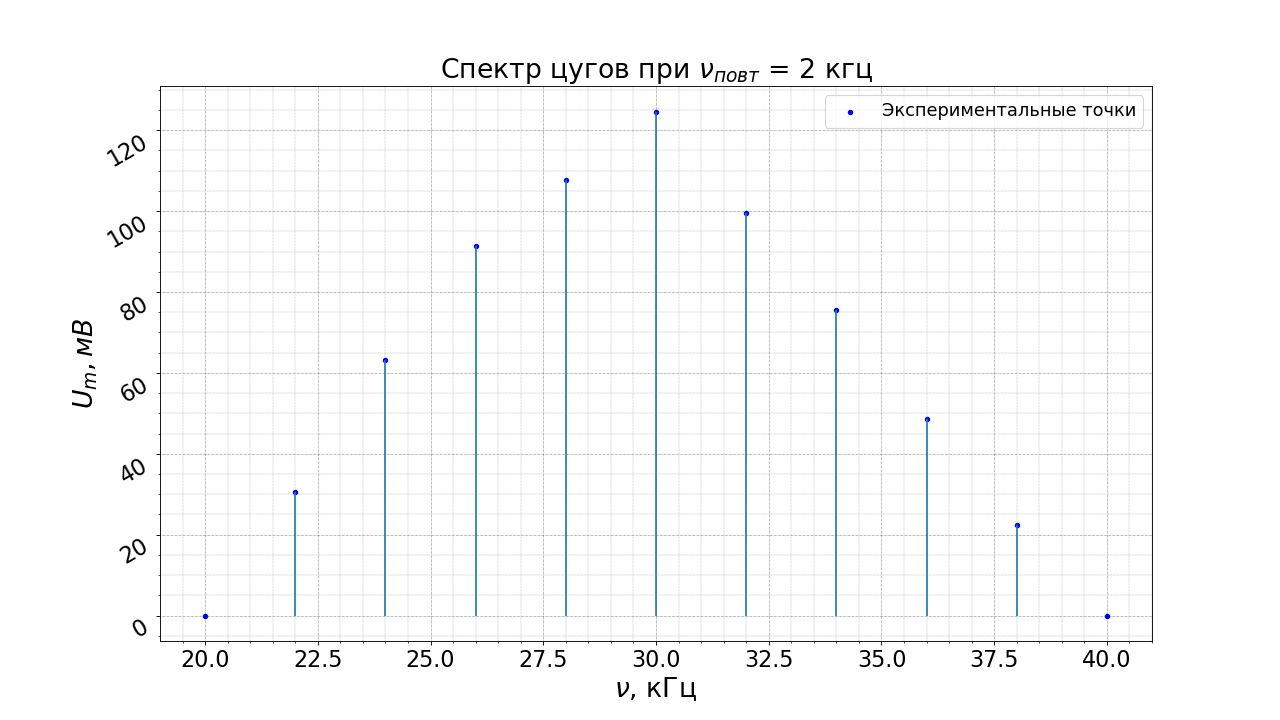
\includegraphics[width = \textwidth]{images/graph_5.png}
        \end{center}

        \noindent\hypertarget{graph_6}{\textbf{График 6. Зависимость отношения амплитуды боковых колебаний к амплитуде несущего колебания от глубины модуляции}}
        \begin{center}
            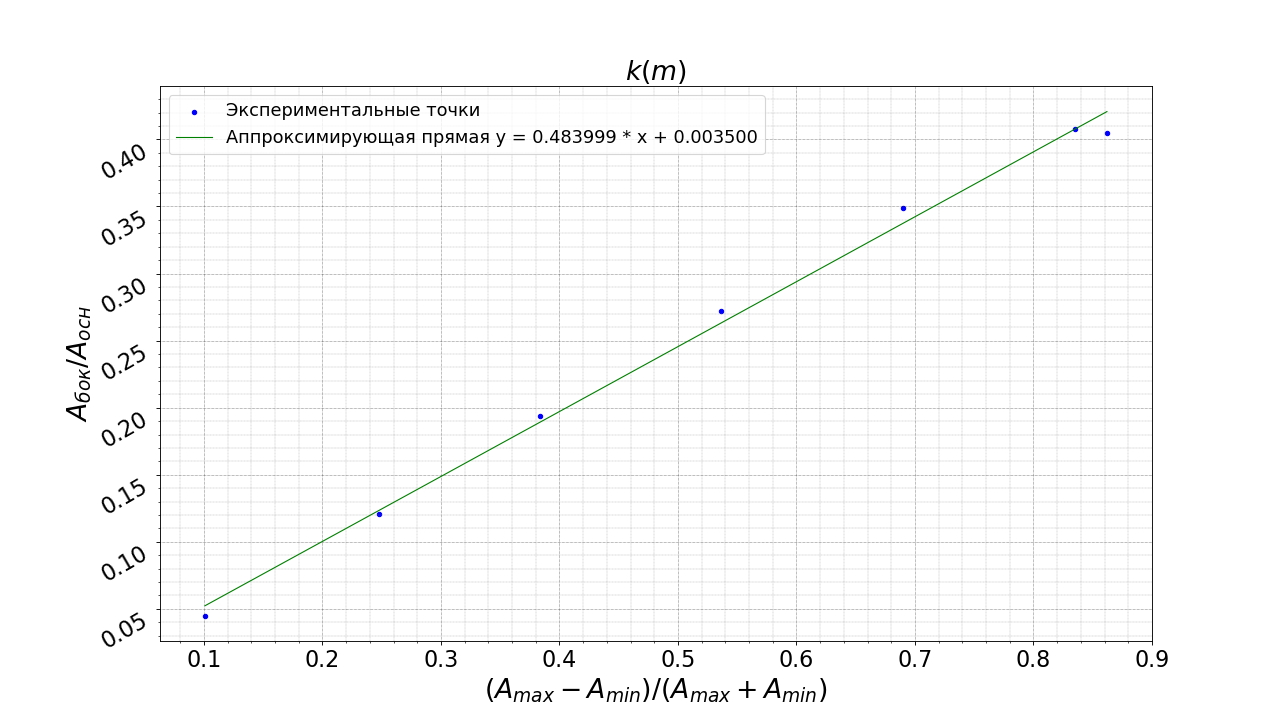
\includegraphics[width = 0.9\textwidth]{images/graph_6.png}
        \end{center}

\end{document}
